\chapter{Summary and further work}

\label{ch:summary}

\section{Structure properties and intrinsic defects in \zirconia}

DFT calculations of non-defective \zirconia\ predicted the correct order of phase stability for the monoclinic, tetragonal and cubic phases. Calculated lattice parameters of each phase also agreed to within 2\% of experimental values. Calculated band gaps of each phase were underestimated by approximately 2 eV, which is typical when modelling using GGA-DFT. A Hubbard +U study revealed that the calculated band gaps could be increased by up to 1 eV, but that the symmetry of the supercells would be distorted in the process.

Helmholtz free energy calculations at temperatures ranging from 0 to 2500 K showed that the lowest energy phase changes from monoclinic to tetragonal, but not from tetragonal to cubic. Furthermore, the predicted transition temperature of the monoclinic-tetragonal phase change is underestimated by almost 1100 K. This is attributed to the kinetic barrier of the phase transformation and the lack of thermal expansion when using the constant volume harmonic model.

Elastic constants were calculated and reported for each phase. The cubic phase was predicted to have the highest stiffness, followed by monoclinic and then tetragonal. The elastic constants were used to calculate the bulk modulus of each phase, and it was shown that the monoclinic and tetragonal bulk moduli agreed with experimental values to within 5\%. The calculated bulk modulus in the cubic phase could not be compared to an experimental value in pure \zirconia , but was 15\% larger than that of YSZ.

\section{Iodine doping and oxygen competition}

\section{Tellurium decay chain elements in \zirconia}

\section{Further work}

\subsection{Fission product empirical potential}

In order to study the interaction of fission products with larger features in the cladding microstructure, such as dislocations and grain boundaries, it is necessary to develop empirical potentials for use in molecular dynamics simulations. Grain boundary transport is of particular interest, and this would require something on the order of 10$^{4}$ atoms to simulate to a reasonable degree of accuracy. This cannot be done using DFT currently due to the significant amount of computing resources required to run such a simulation. 

The development of an iodine and xenon potential with \zirconia\ should be prioritised in order to run simulations to determine the migration of iodine within \zirconia, followed by the behaviour of xenon at sites occupied by iodine.

\subsection{Zr/ZrO/\zirconia\ interface study}

The inner oxide is not a homogeneous structure, as described in § \ref{ch:crystallography}. Figure \ref{fig:zro_interface} clearly shows the existence of a ZrO phase up to 200 nm thick at the interface between \zirconia\ and Zr metal. The presence of ZrO and even oxygen-saturated Zr metal will have an effect on the thermodynamic equilibria of different fission products. An interface study can be conducted using DFT, to determine stresses at the interfaces of Zr and ZrO, and ZrO and \zirconia . Studying the aggregate effect of these interfaces on fission product behaviour may require larger molecular dynamics simulations, however. 

The crystal structure of the ZrO phase has been studied using both simulation and high-resolution electron microscopy, with two likely crystal structures being proposed \cite{Nicholls2015}. Further atomistic studies must be conducted to determine the stability of each crystal structure of ZrO when constrained by \zirconia\ and oxygen-saturated Zr metal interfaces.

\begin{figure}[ht] % ZrO interface
    \centering
    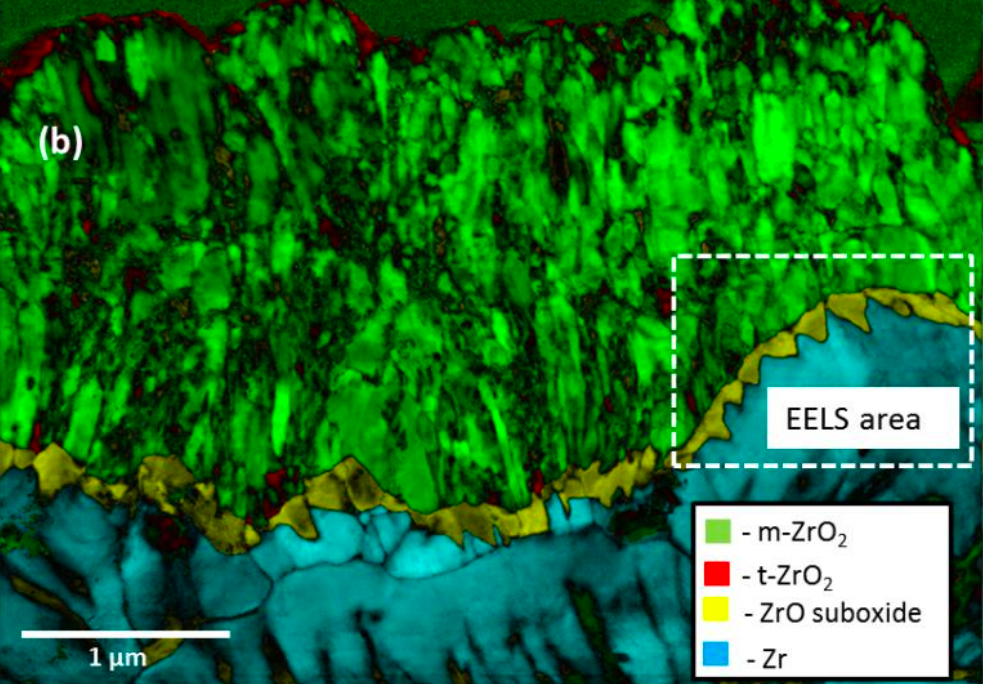
\includegraphics[height=9cm]{images/zro_interface.png}
    \caption[STEM image of a Zr-1.0\%Nb sample oxidised in simulated PWR water at 360 C for 120 days.]{STEM image of a Zr-1.0\%Nb sample oxidised in simulated PWR water at 360 C for 120 days. Taken from \cite{inproceedings}.}
    \label{fig:zro_interface}
\end{figure}

\subsubsection{Bromine}

\subsection{Experimental work}

\subsubsection{Tetragonal phase stabilisation}

A key finding in this thesis is that tetragonal phase \zirconia\ (as opposed to monoclinic) provides the barrier effect against corrosive fission products. It would therefore be useful to conduct experiments on claddings designed to maximise the content of tetragonal phase \zirconia\ in the internal oxide layer. While this can be achieved with a tetragonal stabilising dopant (e.g. scandium, yttrium), this will increase the concentration of oxygen vacancies which may lead to reduced corrosion performance. 

Another method is to increase the amount of tetragonal phase in the oxide layer is to reduce the Zr grain size. This is an attractive option because the chemical composition of the cladding will be unchanged, and the increased strength does not come at the cost of ductility. 

\subsubsection{Oxygen environment control}

In-pile irradiation tests (e.g. power ramps, high burn-up behaviour) to examine the effect of increasing the oxygen content in fuel pins would provide useful data on PCI performance. Presently, fuel pins are filled with helium because it is an inert gas, it does not affect the neutronics within the core and has a high thermal conductivity compared to other gases. One option for varying oxygen content in a fuel pin is to use a fill gas which is a mixture of helium and oxygen. 

Although oxygen (most of which is \ch{O^{16}_{8}}) is not inert and has a lower thermal conductivity than helium, it is highly resistant to neutron activation due to a combination of very low thermal neutron absorption cross-section and three stable isotopes (i.e. three consecutive neutron captures are required to produce an unstable \ch{O^{19}_{8}} nucleus). Adding oxygen to the fill gas is also a much simpler (and therefore cheaper) method of increasing oxygen content compared to changing the stoichiometry of the fuel.

